% % % % % % % % % % % % % % % % % % % % % % % % % % % % % % % % % % % % 
% 
% FS-Vorlage											Stand: 30.01.12
%
% Formelsammlungsvorlage von Emanuel Regnath und Martin Zellner	
% Bietet verschiedene Abkürzungen und Befehle	
%
% % % % % % % % % % % % % % % % % % % % % % % % % % % % % % % % % % % % 


% Dokumenteinstellungen
% ======================================================================

% Dokumentklasse (Schriftgröße 6, DIN A4, Artikel)
\documentclass[6pt,a4paper]{scrartcl}


% Pakete laden
\usepackage[utf8]{inputenc}		% Zeichenkodierung: UTF-8 (für Umlaute)   
\usepackage[german]{babel}		% Deutsche Sprache
\usepackage{multicol}			% ermöglicht Seitenspalten  
\usepackage{longtable}
\usepackage{booktabs}			% bessere Tabellenlinien
\usepackage{graphicx}			% Zum Bilder einfügen benötigt
\usepackage{pbox}				% Intelligent parbox: \pbox{maximum width}{blabalbalb \\ blabal}
\usepackage{scientific}	% Eigenes Paket
\usepackage{parskip}
\usepackage{scrtime}
\usepackage{titlesec}
\usepackage{color}				% Ermöglicht farbigen Text
\usepackage{tabularx}			% Tabellen mit Zeilenumbruch
\usepackage{tikz}				% Alle möglichen Zeichnungen
\usepackage{multirow}                           %zeilenübergreifender Text

% .:: Seitenlayout und Ränder
% ======================================================================
\usepackage{geometry}
\geometry{a4paper,landscape, left=6mm,right=6mm, top=0mm, bottom=3mm,includeheadfoot} 
\definecolor{darkgreen}{rgb}{0,0.5,0}

% .:: Kopf- und Fußzeile
% ======================================================================
\usepackage{fancyhdr}
\pagestyle{fancy}
\fancyhf{}

   \fancyfoot[C]{von Hendrik Böttcher}
   \renewcommand{\headrulewidth}{0.0pt} %obere Linie ausblenden
   \renewcommand{\footrulewidth}{0.1pt} %obere Linie ausblenden

   \fancyfoot[R]{Stand: \today \ um \thistime \ Uhr \qquad \thepage}
   \fancyfoot[L]{Homepage: www.latex4ei.de -- Fehler bitte sofort an info@latex4ei.de}
	
% Schriftart SANS für bessere Lesbarkeit bei kleiner Schrift
\renewcommand{\familydefault}{\sfdefault} 
% Array- und Tabellenabstände vergrößern
\renewcommand{\arraystretch}{1.2}

%\renewcommand{\vec}[1]{\ensuremath{\boldsymbol {#1}}}
%\renewcommand{\ma}[1]{\ensuremath{\boldsymbol {#1}}}

% .:: Überschriften anpassen
% ======================================================================
\definecolor{sectioncolor}{RGB}{40,40,128}

%\titleformat{ command }[ shape ]{ format }{ label }{ sep }{ before-code }[ after-code ]
\titleformat{\section}{\Large \bfseries}{\thesection .}{0.5em}{\color{sectioncolor}}[\color{sectioncolor} \hrule \hrule]
\titleformat{\subsection}{\large \bfseries}{\thesubsection .}{0.3em}{}[ ]

%\titlespacing{Überschriftart}{keine Ahnung}{Abstand oberhalb}{Abstand unterhalb}
\titlespacing{\section}{0em}{1.0em}{0.1em}
\titlespacing{\subsection}{0em}{0.2em}{-0.4em}
\titlespacing{\subsubsection}{0em}{0em}{-0.5em}



% Dokumentbeginn
% ======================================================================
\begin{document}


% Aufteilung in Spalten
\vspace{-3mm}
\begin{multicols}{4}
	\parbox{2.3cm}{
		
\includegraphics[height=1.4cm]{./img/Logo.pdf}		
	}
	\parbox{4cm}{
		\emph{\Large{Mensch-Maschine-Kommunikation 2}}
	}
\vspace{-3mm} % Man muss optimieren wos nur geht ;)
% -------------------------------------------
% | 		MMK 2				|
% ~~~~~~~~~~~~~~~~~~~~~~~~~~~~~~~~~~~~~~~~~~~
%=======================================================================

%\paragraph{Allgemeines}
%el.mag. Wellen transversal, $\bot$ zur Ausbr.richtung, $B\times E$; Schallwellen longitudinale Druckwellen, $\parallel$ zur Ausbr.richtung; 

%Oktave: "`Frequenzverhältnis 1:2"`

%%%%%%%%%%%%%%%%%%%%%%%%%%%%
\section{Allgemeines}
%%%%%%%%%%%%%%%%%%%%%%%%%%%%

\emphbox{Vorverarbeitung - Merkmalsextraktion - Erkennung - Training}

\sectionbox{
%\subsection{Faltung}
%\subsubsection{2D-Faltung}
%	$g(x_1,x_2) * h(x_1,x_2) = \int \limits_{-\infty}^{\infty} \int \limits_{-\infty}^{\infty} g(\xi_1,\xi_2) h(x_1-\xi_1, x_2-\xi_2) \diff \xi_1 \diff \xi_2$

\subsection{2D-Fouriertransformation}
	$G_c(\omega_1, \omega_2) = \int \limits_{- \infty}^{\infty} \int \limits_{- \infty}^{\infty} g(x_1, x_2)  e^{-j \cdot (\omega_1 x_1 + \omega_2 x_2)} \diff x_1 \diff x_2$
	
	\tablebox{
	\begin{tabular*}{\columnwidth}{@{\extracolsep\fill}ccc@{}}
	\ctrule
	$g(x_1, x_2)$ & & $G_c(\omega_1, \omega_2)$ \\
	\cmrule
	$g(ax_1,b x_2), \text{(a,b reel)}$ && $\frac{1}{|ab|} G_c(\frac{\omega_1}{a}, \frac{\omega_2}{b})$ \\
	$g(x_1-a, x_2-b), \text{(a,b reel)}$ & & $ e^{-j \cdot (\omega_1 a+ \omega_2 b)} G_c(\omega_1, \omega_2)$\\
	$ e^{-j \cdot (a x_1 + b x_2)} g(x_1, x_2)$ && $G_c(\omega_1-a, \omega_2-b)$\\
	$\frac{\partial^m}{\partial x_1^m} \frac{\partial^n}{\partial x_2^n} g(x_1, x_2)$&& $(j\omega_1)^m(j\omega_2)^n G_c(\omega_1, \omega_2)$\\
	$(-j\omega_1)^m(-j\omega_2)^n g(x_1, x_2)$ && $\frac{\partial^m}{\partial \omega_1^m} \frac{\partial^n}{\partial \omega_2^n} G_c(\omega_1, \omega_2)$\\
	$G_c(x_1, x_2)$ && $(2\pi)^2 g(-\omega_1, -\omega_2)$\\
	\cmrule
	$\delta(x_1-a, x_2-b) = $ &&  \multirow{2}{*}{$ e^{-j \cdot (\omega_1 a+ \omega_2 b)}$}\\
	$ = \delta(x_1-a)\delta(x_2-b)$ &&\\
	$\frac{1}{4\pi\sqrt{ab}}e^{-(\frac{x_1^2}{4a}+\frac{x_2^2}{4b})}$, (a,b$>$0) && $ e^{-j \cdot (\omega_1^2 a+ \omega_2^2 b)}$\\
	$\begin{cases} 1 & \text{für} |x_1| < a, |x_2| < b \\ 0 & \text{sonst} \end{cases}$ && $4 \frac{\sin(a\omega_1) \sin(b\omega_2)}{\omega_1 \omega_2}$\\
	$\begin{cases} 1 & \text{für} |x_1| < a \\ 0 & \text{sonst} \end{cases}$  && $2 \frac{\sin(a \omega_1)}{\omega_1} \delta(\omega_2)$\\
	\cbrule
	\end{tabular*}
	}

}

\sectionbox{
\subsection{Klassifikation}
\begin{tabular}{l|c|c}
Erkennung & X vorhanden & X nicht vorhanden \\ \hline
X erkannt & \textcolor{darkgreen}{a) richtig positiv} & \textcolor{red}{b) falsch positiv} \\ \hline
X nicht erkannt & \textcolor{red}{c) falsch negativ} & \textcolor{darkgreen}{d) richtig negativ}\\ 
\end{tabular}

%$a_j = \sum \limits_{i=1}^{N_{pos}} sgn(h_j(b_{pos,i}[n_1,n_2])+1)$
}


\sectionbox{
\subsection{Farbräume}
\subsubsection{RGB}
$\mat{R \\ G \\ B} = \mat{ 1 & 0 & 1.140 \\ 1 & -0.395 & -0.581 \\ 1 & 2.033 & 0} \mat{Y \\ U \\ V}$
\subsubsection{YUV}
	\parbox{3cm}{
	Y: Chrominanz (Helligkeit)\\
	U, V: Luminanz (Farbe)\\
	}
	\parbox{3cm}{
	$U = 0.492 \cdot (B - Y)$\\
	$V = 0.877 \cdot (R - Y)$\\
	}

$\mat{Y \\ U \\ V} = \mat{ 0.299 & 0.587 & 0.114 \\ -0.147 & -0.289 & 0.436 \\ 0.615 & -0.515 & -0.1} \mat{R \\ G \\ B}$
\subsubsection{HSV (nicht blau, weiß und schwarz!!!)}
H: Farbton (hue) \\
S: Sättigung (saturation)\\ 
V: Farbwert (value) \\

$V = \max\{R,G,B\}$ ,
 $S =\begin{cases}
 0 & \text{ für } V = 0 \\
 \frac{V- \min\{R,G,B\}}{V} & \text{ sonst.}
 \end{cases}$

$H = \begin{cases}
  \frac{G-B}{V- \min\{R,G,B\}}& \text{ für } V = R, S \neq 0\\
2+ \frac{B-R}{V- \min\{R,G,B\}} & \text{ für } V = G, S \neq 0 \\
4+  \frac{R-G}{V- \min\{R,G,B\}} & \text{ für } V = B, S \neq 0 \\
0 &   \text{ sonst.}
 \end{cases} $
}

\sectionbox{
\subsection{Hauptachsentransformation / PCA}
Zweck: Reduktion der Merkmale durch Verwendung der repäsentativsten Hauptachsen, geringer Rechenaufwand
	\cooknumbox{Berechnung}{
		\item Mittelwert der Punkte: $\vec{\ol a}  = \frac{1}{M}\sum \limits_{i=1}^{M} \vec a_i$
		\item Mittelwertbefreites Essemble: $\ma \Psi = [(\vec a_1 - \vec{\ol a}),...,(\vec a_M - \vec{\ol a})$
		\item Kovarianzmatirix: $\ma \Phi = \frac{1}{M} \ma \Psi \ma \Psi^T$
		\item Eigenwerte: $\det(\ma \Phi - \lambda \cdot \ma I) = 0$
		\item Eigenvektoren: $\ma \Phi \cdot \vec u_k = \vec u_k \cdot \lambda_k \Ra (\ma \Phi - \lambda_k \cdot \ma I) \vec u_k = 0$
		\item Eigenvektoren normieren $\Ra$ Eigenvektoren sind orthogonal
	}
}

%\vfill
%\columnbreak

%%%%%%%%%%%%%%%%%%%%%%%%
\section{Handschrifterkennung}
%%%%%%%%%%%%%%%%%%%%%%%%
\sectionbox{
	\subsection{Vorverarbeitung}
		\cookbox{Eingabemethoden}{
			\item freie Eingabe (hohe Vorverarbeitung)
			\item liniengeführte Eingabe
			\item feldgeführte Eingabe
		}
	Eingangssignal: $\vec x(t) = (x(t), y(t), p(t))^T$\\
	\tablebox{
		\begin{tabular*}{\columnwidth}{@{\extracolsep\fill}ll@{}}
			\ctrule
			x(t) & x-Koordinate\\
			y(t) & y-Koordinate\\
			p(t) & Druck (des Stifts)\\
			\cbrule 
		\end{tabular*}
	}
	
		\subsubsection{Abtastung}
			\cooknumbox{Abtastung / Neuabtastung}{
				\item Diskretisierung von $\vec x(t)$ mit $n \cdot \Delta T \Ra $ zeitäquidistante Abtastung
				\item Lineare Interpolation der Stifttrajektorie
				\item Neuabtastung $\Ra$ ortsäquidistante Abtastpunkte $\vec x_{re}[k]$
			}

			Länge einer Kurve $\vec r(t) = (x(t),y(t))^T$:\\
			$L(a,b) = \int \limits_a^b \sqrt{(\frac{\diff x(t)}{\diff t})^2 + (\frac{\diff y(t)}{\diff t})^2} \diff t$\\
		

		\subsubsection{Korrekturen}
			\cooknumbox{Zeilenneigung (skew)}{
				\item Horizontale Ausrichtung der Kernlinie des Geschriebenen
				\item Drehung um den Mittelpunkt $\vec m$ d. Kernlinie um den Winkel $\alpha_0$
				\item Bestimmung von $\alpha_0$ mit Projektionsprofilen oder Richtungshistogrammen in y-Richtung, $H_y(\alpha)$ muss möglichst klein sein
			}

			Entropie: (B: Anzahl d. Bins, N($B_i$): Anzahl d. Punkte in Bin i)\\
			$H_y(\alpha) = \sum\limits_{i=1}^{B}I(i)$\\
			$I(B_i) = - \frac{N(B_i)}{\sum\limits_{j=1}^{B} N(B_j)} \text(ld) \frac{N(B_i)}{\sum\limits_{j=1}^{B} N(B_j)}$\\
			Regressionsgerade $y = mx+b$:\\
			$m=\frac{\sum \limits_{i=1}^{N}[(x_i - \ol x) (y_i - \ol y)]}{\sum \limits_{i=1}^{N} (x_i - \ol x)^2}$ und $b= \ol y - m \ol x$\\
			Rotation:\\
			$\vec x_{skew}[k] = \mat{ \cos \alpha_0 & -\sin \alpha_0 & 0 \\ \sin \alpha_0 & \cos \alpha_0 & 0 \\ 0&0&1} (\vec x_{re}[k] - \vec m)+ \vec m$\\
			

			\cooknumbox{Schriftneigung (slant)}{
				\item Scherung der Schrift an der Grundlinie $y_S$
				\item Scherung um den Winkel $\phi_0$
				\item Bestimmun von  $\phi_0$ mit  Projektionsprofilen oder Richtungshistogrammen in x-Richtung, $H_x(\phi)$ muss möglichst klein sein
			}

}

\sectionbox{

			Scherung:\\
			$\vec x_{slant}[k] = \mat{ 1 & -\tan\phi_0 & 0 \\ 0& 1 & 0\\ 0 & 0 & 1} (\vec x_{skew}[k]- \mat{0 \\ y_S \\ 0})+ \mat{0 \\ y_S \\ 0}$ \\
		
			\cooknumbox{Schriftgröße}{
				\item Schätzen der Referenzlinien
				\item Berechnung der Kernhöhe
				\item Normirung des Schriftzuges
			}
			
			W: Höhe der Bins, P: Projektionsprofil\\
			Oberlängenlinie: $y_{ober} = y_{max}$, Unterlängenlinie: $y_{unter} = y_{min}$\\
			Kernlinie: $y_{kern}  = \text{argmin}(\frac{\diff}{\diff j}P_y(j))-0.5)W+ y_{min}$\\
			Basislinie: $y_{grund} = \text{argmax}(\frac{\diff}{\diff j}P_y(j))-0.5)W+ y_{min}$\\
			Kernhöhe: $h_{kern} = |y_{kern}-y_{grund}|$\\
			Normierung:\\
			$\vec x_{norm}[k] = \frac{1}{h_{kern}} \mat{x[k] - x_{min} \\ y[k] - (y_{grund} + \frac{h_{kern}}{2})}$
}

\sectionbox{
	\subsection{Merkmalsextraktion}
		Extraktion aus dem normalisierten Schriftzug\\
		Sekantensteigungswinkel:\\
		$\theta[k] = \frac{\pi}{2} + \begin{cases}\arctan(\frac{\Delta y}{\Delta x}) - \frac{\pi}{2} \sgn(\Delta x) & \text{für } \Delta x \neq 0\\
								     \frac{\pi}{2} (1- \sgn(\Delta x) ) & \text{für } \Delta x = 0 \end{cases}$\\
$\Delta x = x_{norm}[k+1]-x_{norm}[k]$, $\Delta y = y_{norm}[k+1]-y_{norm}[k]$\\
		Richtungsänderung:\\
		$\Delta \theta[k] = \theta[k+1]-\theta[k]$\\
		5-dim. Merkmalsvektor:
		$\vec m[k] = \mat{\sin(\theta[k]) \\ \cos(\theta[k]) \\ \sin(\Delta \theta[k]) \\ \cos(\Delta \theta[k]) \\ p[k]}$

}

\sectionbox{
	\subsection{Erkennung}
		Trainig und Erkennung läuft über Hidden-Markov-Modelle (HMM) mit Graphemen (z.B. Buchstabe, Sonderzeichen od. Ziffern) als kleinste Einheit\\
		Training: Baum-Welch-Alogrithmus\\
		Erkennung: Viterbi-Algorithmus\\
}

%%%%%%%%%%%%%%%%%%%%%%%%%%%%%%%%%
\section{Bildverarbeitung}
%%%%%%%%%%%%%%%%%%%%%%%%%%%%%%%%%

\sectionbox{
\subsection{Separierbarkeit}
	Das Signal $g(x_1,x_2)$ lässt sich schreiben als:\\
	\emphbox{
	$g(x_1,x_2) = g_1(x_1) \cdot g_2(x_2)$
	}
	Bildfilter möglichst immer separieren, um Laufzeit bzw. Operationen zu sparen.
}


\sectionbox{
\subsection{Diskrete Signale}	

\subsubsection{Kausalität}
kausal, wenn: $g[n_1,n_2] = \begin{cases} \text{beliebig} & \text{für} n_1,n_2 > 0\\
							0 & \text{sonst.}\end{cases}$

\subsubsection{Abtastung}
Abtastabstände: $X_1, X_2$\\
Abtastheorem: $\frac{\pi}{X_1} \ge \omega_{g,1}$ und $\frac{\pi}{X_2} \ge \omega_{g,2}$\\
 Grenzfrequenz $\omega_{g,i}$: maximal vorkommende Frequenz in Richtung $\omega_i$

\subsubsection{Quantisierung}
normalerweise lineare Quantisierung mit $N=2^b$ Stufen. (b: \#Bits)\\
fürs menschliche Auge genügen 256 Graustufen

\subsubsection{Dynamikbereich}
Bereich zwischen dem gößten ($g_{max}$) und kleinsten Grauwert ($g_{min}$) 

}

\sectionbox{

\subsubsection{Speicherbedarf von Grauwertbildern}
\# Bits für Dynamikbereich:$ b = \lceil \text{ld} (g_{max}-g_{min}+1) \rceil$\\
M: \#Zeilen, N: \#Spalten\\
Speicherplatz: $b \cdot M \cdot N$



\subsubsection{Z-Transformation}
$G(z_1,z_2) = \sum \limits_{n_1 = - \infty}^{\infty} \sum \limits_{n_2 = - \infty}^{\infty} g[n_1, n_2] z_1^{-n_1} z_2^{-n_2}$\\
	\tablebox{
	\begin{tabular*}{\columnwidth}{@{\extracolsep\fill}cc@{}}
	\ctrule
	$g[n_1, n_2]$ & $G(z_1,z_2)$\\
	\cmrule
	$\delta[n_1,n_2]$ & $1$\\
	$\delta[n_1-a,n_2-b]$ & $z_1^{-a}z_2^{-b}$\\
	\cbrule
	\end{tabular*}
	}\\


	\cooknumbox{Von der Filtermatrix zur Übertragungsfunktion}{
		\item Filtermatrix: $\mat{1 & 0 & 0 \\ 0 & 2 & 3 \\ \textcolor{red}{\emph{-1}} & 0 & 0 }$ \\
		\item Impulsantwort: $g[n_1,n_2] =\\ =  -\delta[n_1,n_2] + 2 \delta[n_1-1, n_2-1] + 3 \delta[n_1-2, n_2-1]+\\ + \delta[n_1, n_2-2]$\\
		\item Übertragungsfunktion: $G(z_1,z_2) = \\ =  -1 + 2 z_1^{-1}z_2^{-1}+ 3 z_1^{-2} z_2^{-1} + z_2^{-2}$\\
	}

\subsubsection{Filterstukturen}
	$H(z) = \frac{Y(z)}{X(z)} = \frac{b_0+b_1z^{-1}+...+b_mz^{-m}}{1+a_1z^{-1}+...+a_mz^{-m}}$\\
	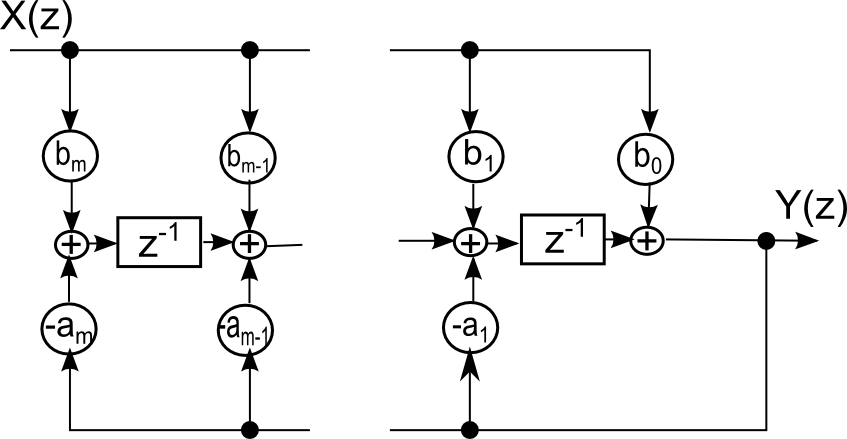
\includegraphics[width=6.9cm]{./img/Filterstruktur.png}

}

\sectionbox{
\subsection{Bildstörungen}
\subsubsection{Additive Bildstörung}

\begin{itemize}
\item weißes, gaußverteiltes Rauschen:\\
	 ensteht durch spontane Ladungstrennung oder thermischen Störung bei der Analog/Digitalwandlung
\item Impulsrauschen ("`Salt'n'Pepper"'): \\
	fehlerhafte Pixel erscheinen als schwarze oder weiße Bildpunkte
\end{itemize}

\subsubsection{Lineare, ortsinvariante Bildstörungen}
\begin{itemize}
\item Motion Blur: \\
	Verwischung durch Bewegung von Objekt oder Sensor
\item Focus Blur:\\
	Unschärfe durch falsche Fokussierung
\end{itemize}
}

\vfill
\columnbreak

\sectionbox{
\subsection{Bildrestauration /-verbesserung}
	\subsubsection{Rauschkompensation}
		\cookbox{Kompensationfilter}{
			\item Mittelwertfilter: $\mat{\frac{1}{9} & \frac{1}{9} & \frac{1}{9} \\ \frac{1}{9} & \frac{1}{9} & \frac{1}{9} \\ \frac{1}{9} & \frac{1}{9} & \frac{1}{9}}$
			\item Gaußfilter (Gaußtiefpass): $\mat{\frac{1}{16} & \frac{1}{8} & \frac{1}{16} \\ \frac{1}{8} & \frac{1}{4} & \frac{1}{8} \\ \frac{1}{16} & \frac{1}{8} & \frac{1}{16}}$
			\item Medianfilter: akt. Pixel bekommt den Wert des Medians der Filtermaske zugewiesen
		}\\

		\symbolbox{
			\paragraph{Median} wird aus auf- oder absteigend geordnetet Werten\\$\vec x = \{x_1, ..., x_N\}$ gebildet.\\
			$\text{Median}(\vec x) =  \begin{cases}
								 x_{\frac{N+1}{2}} & \text{ für N ungerade} \\
								 0.5 \cdot (x_{\frac{N}{2}}+x_{\frac{N+2}{2}}) & \text{ für N gerade}
								 \end{cases}$
		}
	\subsubsection{Blurkompensation}
		Finde raus wie die Störfunktion $H(z_1,z_2)$  aussieht und musltipliziere mit $\frac{1}{H(z_1,z_2)}$  $\Ra$ alles roger.... total einfach... am besten mit dieser Aufgabe anfangen..... NICHT!!!
	\subsubsection{Histogrammausgleich}
		Vorteil: Kontrasterverbesserung \\
		Nachteil: u.u. unnatürliches Bild
	\paragraph{kontinuierlich} $\;$\\
		momentane Verteilung: $p_g$, angestrebte Vereilung: $p_ f$,\\
		 Gesucht: $T_f(g) = f$\\
		$\int \limits_0^f p_f(f_0)\diff f_0 \overset{!}{=} \int \limits_0^g p_g(g_0)\diff g_0$ \\
		bei angestrebter Gleichverteilung: $T_f(g) = f = \int \limits_0^g p_g(g_0)\diff g_0$
	\paragraph{diskret}$\;$\\
	$T(g) = \underset{0\le g_{norm} \le G-1}{\text{argmin}} |K_b(g)-K_{b,norm}(g_{norm})|$

}

\sectionbox{
\subsection{Kantenhervorhebung}
	\parbox{4cm}{
	\textcolor{red}{\emph{akt. Pixel}} ist \textcolor{red}{rot} und \emph{fett}
	}
	\parbox{1cm}{
	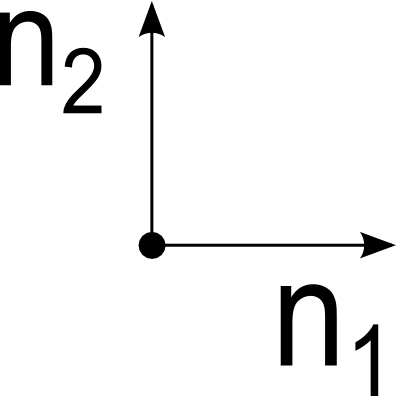
\includegraphics[width=1cm]{./img/n1n2_System.png}
	}

	\subsubsection{Gradientenfilter in $n_1$-Richtung}
	Detektion harter Kanten\\
	Pixeldifferenz: $\mat{ \textcolor{red}{\emph{1}} & -1}$ 
	separ. Pixeldiff.: $\mat{1 & \textcolor{red}{\emph{0}} & -1} $\\
	Prewitt: $\mat{1 & 0 & -1 \\ 1 & \textcolor{red}{\emph{0}} & -1 \\ 1 & 0 & -1 }$ 
	Sobel: $\mat{1 & 0 & -1 \\ 2 & \textcolor{red}{\emph{0}} & -2 \\ 1 & 0 & -1 }$ \\
	Frei-Chen: $\mat{1 & 0 & -1 \\ \sqrt{2} & \textcolor{red}{\emph{0}} & -\sqrt{2} \\ 1 & 0 & -1 }$ 

	\subsubsection{Gradientenfilter in $n_1$-Richtung}
	Detektion harter Kanten\\
	Pixeldifferenz: $\mat{ -1 \\ \textcolor{red}{\emph{1}}}$ 
	separ. Pixeldiff.: $\mat{-1 \\ \textcolor{red}{\emph{0}} \\ 1} $\\
	Prewitt: $\mat{1 & 1 & 1 \\ 0 & \textcolor{red}{\emph{0}} & 0 \\ -1 & -1 & -1 }$ 
	Sobel: $\mat{1 & 2 & 1 \\ 0 & \textcolor{red}{\emph{0}} & 0 \\ -1 & -2 & -1 }$ \\
	Frei-Chen: $\mat{1 & \sqrt{2} & -1 \\ 0 & \textcolor{red}{\emph{0}} & 0 \\ -1 & -\sqrt{2} & -1 }$ 

}

\sectionbox{

	\subsubsection{Laplacefilter}
	Detektion weicher Kanten\\
	$\mat{0 & -1 & 0 \\ -1 & \textcolor{red}{\emph{4}} & -1 \\ 0 & -1 & 0 }$ 
	$\mat{-1 & -1 & -1 \\ -1 & \textcolor{red}{\emph{8}} & -1 \\ -1 & -1 & -1 }$ 
	$\mat{1 & -2 & 1 \\ -2 & \textcolor{red}{\emph{4}} & -2 \\ 1 & -2 & 1 }$ 
	%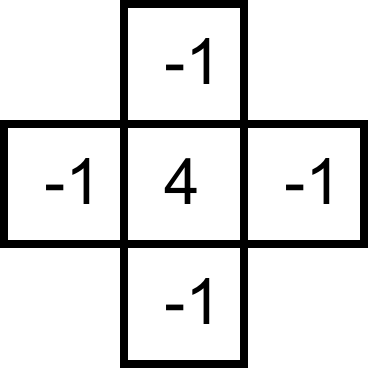
\includegraphics[height=1.4cm]{./img/laplaceFilter.png}
	\subsubsection{Binarisierung}
	weitere Herausarbeitung der Kanten z.B für anschließende Segmentierung oder Skelettierung\\
	$b_{Bin}[n_1,n_2] = \begin{cases}
		1 & \text{für } b[n_1,n_2] \ge s\\
		0 & \text{für } b[n_1,n_2] < s\\
		\end{cases}$\\
	s ist die Entscheiderschwelle. Meist ist $s<50$
	%$\Delta b_t[n_1,n_2] = 
	%	\left\{ \begin{aligned}
	 %1 & \text{ für } |b_t[n_1,n_2]-b_r[n_1,n_2]| > s \\
	 %0 & \text{ sonst.}
	 %\end{aligned} \right.$
}

\sectionbox{
\subsection{Morphologische Operatoren}
 Anwendung auf Binärbilder mit kleinen Strukturelementen.\\
Vergleich des aktuellen Pixels und Umgebung mit dem Muster des Strukturelements
	\subsubsection{Erosion}
		komplettes Muster stimmt  mit der Umgebung des akt. Pixels überein\\ $\Ra$ akt. Pixel ist 1
		(Fläche nimmt ab)
	\subsubsection{Dilatation}
		ein Teil des Musters stimmt mit der Umgebung des akt. Pixels überein\\ $\Ra$ akt. Pixel ist 1
		(Fläche nimmt zu)
	\subsubsection{Öffnen}
		Erosion, dann Dilatation\\
		(Unruhige Teile des Bildes werden entfernt)
	\subsubsection{Schließen}
		Dilatation, dann Erosion\\
		(kleine, getrennt liegende Teile werde zu einem größeren Objekt zusammengefasst)
}

\section{Gesichtsdetektion}
\emphbox{
Gesichter werden auf Bildern erkannt.
}

\sectionbox{
\subsection{Farbbasierte Gesichtsdetektion}
\emph{Hautfarbensegmentierung:} Analyse sehr vieler verschiedener Gesichter\\
\emph{typische Farbwerte für Gesichter im HSV-Raum:}\\
 $0 \le H \le 36^{\circ}$ und $0,1 \le S \le 0.57 $\\
\Ra Binarisierung der Gesichtsbilder \\
\emph{Fazit:} eignet sich für genauere Überprüfungen von erkannten Gesichtern aus anderen Verfahren
}

\sectionbox{
\subsection{Multiskalen-basierte Gesichtsdetektion}
Skalierte Bilder, um verschiedene Blockgrößen für unterschiedliche Gesichtsgrößen erhalten zu können \\
Tiefpassfilterung des Bildes\\
Unterabtastung um den Faktor 2 $\Ra \frac{N}{4}$ neue Bildpunkte \\
Speicherung: $N_{ges} = \frac{4}{3} \cdot N$ (geomtr. Reihe) \\
}

\vfill
\columnbreak

\sectionbox{
\subsection{Viola-Jones}
ist formbasiert\\
hohe Erkennungsrate und geringe Rechenzeit für Detektion\\
\subsubsection{Merkmale}
	Allgemeine Form: $m_s\cdot m \times n_s \cdot n$\\
	\tablebox{
	\begin{tabular*}{\columnwidth}{@{\extracolsep\fill}lccc@{}}
	\ctrule
	 \multirow{2}{*}{Typ}  & \multirow{2}{*}{Basis} & min. Höhe& min. Breite\\
	 & &  ($m_s\cdot m$) &  ($n_s\cdot n$)\\
	\cmrule
	A & $\mat{1 & -1}$ & $1\cdot m$  & $2\cdot n$\\
	B & $\mat{1 \\ -1}$ & $2 \cdot m$ & $1\cdot n$\\
	C & $\mat{1 & -1 & 1}$ & $1 \cdot m$ & $3\cdot n$\\
	D & $\mat{1 \\ -1 \\ 1}$ & $3 \cdot m$ & $1\cdot n$\\
	E & $\mat{1 & -1 \\ -1 & 1}$ & $2 \cdot m$ & $2 \cdot n$\\
	\cbrule
	\end{tabular*}
	}

\paragraph{max. Skalierung} mit Bild $M \times N$: \\
$m_{max} = \lfloor \frac{M}{m_s} \rfloor$ und $n_{max} = \lfloor \frac{N}{n_s} \rfloor$
\paragraph{Anzahl d. Translationen} in n- und m-Richtung:\\
$N_{m,trans} = M-m_s m +1$ und $N_{n,trans} = N-n_s n +1$

\paragraph{Anzahl d. Realisierungen} $N_{ges}$\\
$N_{ges} = \sum \limits_{n=1}^{n_{max}} \sum \limits_{m=1}^{m_{max}} N_{n,trans} \cdot N_{m,trans} =$\\
$=  \sum \limits_{n=1}^{n_{max}}  N_{n,trans}  \sum \limits_{m=1}^{m_{max}} N_{m,trans} = $\\
$= \frac{n_{max}[2N+2-n_s(n_{max}+1)] \cdot m_{max}[2M+2-m_s(m_{max}+1)]}{4}$\\


\subsubsection{Integralbild}
Integration des Orginalbildes ( Aufsummierung der Pixelwerte bis zum aktuellen Pixel)\\
$b_{int}[n_1,n_2] = \sum \sum b[n_1,n_2]$ mit $1\le n_1 \le  N_1$ , $1 \le n_2 \le N_2$ \\
$\Ra$ Einspaarungen von Operationen: Bei Rechteckfiltern $\Ra$ Reduzierung auf 4 Operationen (Verrechnung der Eckwerte)\\
$\Ra$ Unabhängigkeit von der Merkmalsskalierung\\

	\cooknumbox{Schnelles Aufstellen des Integralbildes}{
		\item Orginalbild:
			$\mat{1 & 1 & 1\\ 1 & 1 & 1\\ 1 & 1 & 1}$
		\item Berechnung d. Spaltensummen:
			$\mat{1 & 1 & 1\\ 2 & 2 & 2\\ 3 & 3 & 3}$
		\item Berechnung d. Zeilensummen:
			$\mat{1 & 2 & 3\\ 2 & 4 & 6\\ 3 & 6 & 9}$
	}

\subsubsection{AdaBoost-Algorithmus}
Maschinelles Lernen zur Merkmalsselektion \& optimale Kombination der selektierten Klassifikatoren \\
viele schwache Klassifikatoren sind zusammen stark\\
macht aus schwachen Klassifikatoren starke Klassifikatoren

\subsubsection{Kaskadierung}
Kaskadierung mehrerer starker Klassifikatoren. Die Komplexität nimmt dabei zu.
}

\vfill
\columnbreak

\section{Gesichtsidentifikation}
\emphbox{
Merkmale von bereits erkannten Gesichtern werden weiterverabeitet
}

\sectionbox{
\subsection{Gesichtserkennung mit Eigengesichtern}
Darstellung von Gesichtsbildern in einem anderen Koordinatensystem duch Hauptachsentransformation\\
Hauptachsen sind Vektoren die selbst als Gesichtsbilder aufgefssst werden können $\Ra$ Eigengesichter\\
starke Reduktion der Dimensionalität möglich\\
dann Abstandsklassifikatoren im reduzierten Merkmalsraum\\
M Gesichtsbilder der Größe $ N_1$x$ N_2$\\
Verfahren siehe PCA(Allgemeines)
}

\sectionbox{
\subsection{Prokrustes Analyse}
Ziel: Möglichst gute Übereinstimmung der zwei Vielecke\\
$\ma P  = [\vec p_1,..., \vec p_N]$ , 
$\ma Q  = [\vec q_1,..., \vec q_N]$ \\
$\ma M(a_x, a_y) = \mat{a_x &  -a_y \\ a_y & a_x} = \ma A_{skal} \cdot \ma A_{rot}$:  Skalierung, Rotation\\
$a_x = s \cos \alpha$, $a_y = s\sin \alpha$\\
$\vec t$: Translation\\
Gewichtungsfaktor$ c_i$ (meistens 1)\\

Minimierung des Quadrates der gewichteten Fehler:\\
$E = \sum \limits_{i=1}^N E_i =  \sum \limits_{i=1}^N c_i |\vec p_i - \ma M(a_x,a_y) [\vec q_i]- \vec t|^2$\\
$\frac{\partial E}{\partial(a_x,a_y,t_x,t_y)}=0 \\
 \Ra \frac{\partial E}{\partial a_x} = 0, \frac{\partial E}{\partial a_y} = 0, \frac{\partial E}{\partial t_x} = 0, \frac{\partial E}{\partial t_y} = 0$\\
$ \mat{Z & 0 & X_q & y_q \\ 0 & Z & -Y_q & X_q \\ X_q & -Y_q & N & 0 \\ Y_q & X_q & 0 & N} \cdot \mat{a_x\\ a_y \\ t_x\\ t_y} = \mat{C_1\\ C_2\\X_p\\ Y_p}$


$X_p = \sum_{i=1}^N c_i \cdot p_{x,i}\\
  Y_p = \sum_{i=1}^N c_i \cdot p_{y,i} \\
X_q = \sum_{i=1}^N c_i \cdot q_{x,i}\\
  Y_q = \sum_{i=1}^N c_i \cdot q_{y,i} \\
Z = \sum_{i=1}^N c_i \cdot (q_{x,i}^2 + q_{y,i}^2)\\
 C = \sum_{i=1}^N c_i \\
C_1 = \sum_{i=1}^N c_i \cdot (p_{x,i} \cdot q_{x,i} + p_{y,i} \cdot q_{y,i}) \\
 C_2 = \sum_{i=1}^N c_i \cdot (p_{y,i} \cdot q_{x,i} - p_{x,i} \cdot q_{y,i})$

$a_x = - \frac{X_p \cdot X_q + Y_p \cdot Y_q - N \cdot C_1}{N \cdot Z - X_q^2 - Y_q^2} \\
a_y = \frac{X_p \cdot X_q - Y_p \cdot Y_q + C \cdot C_2}{N \cdot Z - X_q^2 - Y_q^2} \\
t_x = \frac{X_p \cdot Z - C_1 \cdot X_q + C_2 \cdot Y_q}{N \cdot Z - X_q^2 - Y_q^2} \\
t_y = \frac{Y_p \cdot Z - C_1 \cdot Y_q - C_2 \cdot X_q}{N \cdot Z - X_q^2 - Y_q^2} \\
s  = \sqrt{a_x^2 + a_y^2} \\
 \alpha = \arccos\left(\frac{a_x}{s}\right) = \arcsin\left(\frac{a_y}{s}\right) $\\

}


\sectionbox{
\subsection{Delaunay-Kriterium}
Erfüllt, wenn sich im Umkreis des Dreiecks $\vec a,\vec b ,\vec c$ kein weiterer Punkt $\vec p_x$ befindet. Der Mittelpunkt des Umkreises ist der Schnittpunkt der Seitenhalbierenden.\\

$\vec g = \vec s_a + \lambda \mat{0 & -1 \\ 1 & 0 } (\vec{b} - \vec{a})\\
  \vec{s}_a = \vec{a} + 0.5(\vec{b} - \vec{a}) \\
\vec{h} = \vec{s}_b + \mu \mat{0 & -1 \\ 1 & 0 } (\vec{c} - \vec{a}) \\
 \vec{s}_b = \vec{b} + 0.5(\vec{c} - \vec{b})$

$g = h$ setzen $\Ra$ 2 Geleichungen mit 2 Unbekannten $\mu, \lambda$ $\Ra$ Einsetzen in g oder h $\Ra$ Umkreismittelpunkt $\Ra$ Radius bestimmen
}

%\sectionbox{
%\subsection{Active Shape Models}

%}

%\section{Objektverfolgung}

%\sectionbox{
%\subsection{Differenzbilder}
%$
%\Delta b_t[n_1,n_2] = 
%\begin{cases}
 %1 & \text{ für } |b_t[n_1,n_2]-b_r[n_1,n_2]| > s \\
% 0 & \text{ sonst.}
 %\end{cases}
%$
%}

\end{multicols}

% Dokumentende
% ======================================================================
\end{document}
